\documentclass[a4paper,unicode]{report}
\usepackage{amsmath}
\usepackage{amssymb}
\usepackage{textgreek}
\usepackage{esint}
\usepackage{subfig}
\usepackage{rotating}
\usepackage{booktabs}
\usepackage{longtable}
\usepackage{paralist}
\usepackage{titlesec}
\usepackage{graphicx}
\usepackage{physics}
\usepackage{ucs}
\usepackage{listings}
\usepackage{multirow}
\usepackage{tablefootnote}
\usepackage{indentfirst}
\usepackage{tikz}
\usepackage{warpcol}
\usepackage[pdftitle=计算物理第一次大作业第二部分,pdfauthor=***,bookmarksnumbered=true]{hyperref}
\usepackage{natbib}
\usepackage{xcolor}
\usepackage{xeCJK}
    \setCJKmainfont[BoldFont={Noto Serif CJK SC Bold},ItalicFont={FangSong}]{Noto Serif CJK SC}
    \setCJKsansfont[BoldFont={Noto Sans CJK SC Bold},ItalicFont={KaiTi}]{Noto Sans CJK SC}
    \setCJKmonofont[BoldFont={Noto Sans Mono CJK SC Bold}]{Noto Sans Mono CJK SC}

\title{计算物理第一次大作业第二部分}
\author{物理学院\quad ***\quad 1800011***}

\DeclareUnicodeCharacter{"00B0}{\textdegree}

\renewcommand{\today}{\number\year 年\number\month 月\number\day 日}
\renewcommand{\refname}{参考文献}
\renewcommand{\abstractname}{摘要}
\renewcommand{\contentsname}{目录}
\renewcommand{\figurename}{图}
\renewcommand{\tablename}{表}
\renewcommand{\appendixname}{附录}
\renewcommand{\chaptername}{第}
\newcommand{\chapterendname}{章}

\renewcommand{\equationautorefname}{式}
\renewcommand{\figureautorefname}{图}
\newcommand{\subfigureautorefname}{子图}
\renewcommand{\tableautorefname}{表}
\renewcommand{\subsectionautorefname}{小节}
\newcommand{\mythmautorefname}{定理}
\renewcommand{\sectionautorefname}{\S}

\newtheorem{mythm}{定理}

\lstset{
    basicstyle=\scriptsize\ttfamily\color{black}, % print whole listing small
    keywordstyle=\color{teal}\bfseries,
    identifierstyle=, % nothing happens
    commentstyle=\color{gray}\ttfamily, % white comments
    stringstyle=\color{violet}, % typewriter type for strings
    showstringspaces=true,
    numbers=left,
    numberstyle=\tiny\color{brown},
    stepnumber=2,
    numbersep=5pt,
    firstnumber=auto,
    frame=lines,
    language=[11]C++,
    rangeprefix=/*,
    rangesuffix=*/,
    includerangemarker=false
}

% \pgfsetxvec{\pgfpoint{0.02cm}{0}}
% \pgfsetyvec{\pgfpoint{0}{0.1em}}

% \usetikzlibrary{datavisualization,plotmarks,datavisualization.formats.functions}
% \usetikzlibrary{math,fpu,datavisualization}
% \graphicspath{{figure/}}
\linespread{1.3}

\titleformat{\chapter}[display]{\huge\bfseries}{\chaptertitlename\ \thechapter\ \chapterendname}{20pt}{\Huge}

\begin{document}

\maketitle
\tableofcontents

\begin{center}
    \textbf{编译与运行环境说明}
\end{center}

本地操作系统版本为\textsf{Windows 10 x64 1909 (18363.778)}。

第三、四题使用\textsf{C++}编写,编译器为Windows下的\texttt{g++ 9.3.0} (Rev2, Built by MSYS2 project),标准为\textsf{C++17}。
除标准库外未使用其他第三方库。
最后上交的程序的编译命令为\begin{verbatim}
    g++ -static -std=c++17 -o <可执行文件名> <源文件名>
\end{verbatim}

\setcounter{chapter}{2}
\chapter{Poisson方程}
本题要求使用二阶中心差分求解Poisson方程
\begin{equation}
    \begin{cases}
        -u_{xx} - u_{yy} = 2\pi^2\sin(\pi x)\sin(\pi y),\quad 0<x, y<1;\\
        \eval{u}_{\partial \Omega} = 0, \quad \Omega=(0, 1)\times(0, 1),
    \end{cases}
\end{equation}
并给出$L_2$范数下的误差估计。
两方向差分的剖分数均为$2^n$,分别在$n=4,5,6,7$时求解、比较误差。

容易得到,该方程的解析解为
\begin{equation}
    u(x,y) = \sin(\pi x)\sin(\pi y).
\end{equation}

求解程序为\texttt{3\_Poisson.cpp},主要的求解函数为\texttt{solve<N>()},完成剖分数为$2^N$的全题求解,声明如下
{
    \linespread{1.0}
    \lstinputlisting[linerange=beg:solve_decl-end:solve_decl]{3_Poisson.cpp}
}
参数\texttt{output}为是否输出到文件;\texttt{prefix}为输出文件名的前缀(默认为保存到文件夹\texttt{3\_Poisson})。

函数\texttt{solve<N>()}在正式求解前先做一些初始操作,如下
{
    \linespread{1.0}
    \lstinputlisting[linerange=beg:solve_init-end:solve_init]{3_Poisson.cpp}
}
将剖分数的指数\texttt{N}加入到文件名\texttt{prefix}中;
定义剖分数\texttt{partition},微分算符矩阵边长\texttt{mat\_size},横纵坐标取值范围\texttt{xa, xb, ya, yb}等数个字面量。

\section{求解离散化的Poisson方程}
基本思路为获得拉普拉斯算符$\laplacian$以及非齐次项的离散化形式,然后使用矩阵的迭代法求解矩阵方程。
相关程序如下
{
    \linespread{1.0}
    \lstinputlisting[linerange=end:solve_init-end:prob_1]{3_Poisson.cpp}
}
使用函数\texttt{laplacian<partition, partition>()}(见\autoref{ssec:laplacian})获得以稀疏矩阵存储的$\laplacian$,存入\texttt{op}。
使用函数\texttt{sinxy<partition, partition>()}(见\autoref{ssec:sinxy})获得非齐次项$2\pi^2\sin(\pi x)\sin(\pi y)$,存入\texttt{b}。
使用函数\texttt{suc\_over\_rel()}用超松弛法求解线性方程\begin{equation}
    \text{\texttt{op} \texttt{solution}} = \text{\texttt{b}},
\end{equation}
松弛因子$\omega=1.95$。
最后,将结果输出到文件\texttt{N\_1}(参见文件夹\texttt{3\_Poisson/}中的\texttt{4\_1, 5\_1, 6\_1, 7\_1})。

方程的离散化首先将二维网格上的点编号。
$x$方向用$i$编号,剖分数为$M$;$y$方向用$j$编号,剖分数为$N$;两方向步长分别为$h_x, h_y$。
那么方程离散为
\begin{equation}
    − \frac{u_{i−1,j} − 2u_{i,j} + u_{i+1,j}}{h_x^2}
    − \frac{u_{i,j−1} − 2u_{i,j} + u_{i,j+1}}{h_y^2}
    = f_{i,j} = f(x_i ,y_j).
\end{equation}
且$i, j$取到边界时函数值为0。
将二维网格上的格点按照$y$方向优先遍历(\textsf{C}风格的行优先)压缩到一维,那么拉普拉斯算符的离散化形式为一个\textbf{块三对角矩阵},每一块的大小为$(N-1)\times(N-1)$。
非对角的块均为矩阵$-\frac{I_{(N-1)\times(N-1)}}{h_x^2}$,而对角的块为一个\textbf{三对角矩阵}$A$。
$A$的非对角上的非零元素为$-\frac{1}{h_y^2}$,对角元为$\frac{2}{h_x^2}+\frac{2}{h_y^2}$。

\subsection{获得拉普拉斯算符}\label{ssec:laplacian}
函数\texttt{laplacian<M, N>()}完整定义如下
{
    \linespread{1.0}
    \lstinputlisting[linerange=beg:laplacian-end:laplacian]{3_Poisson.cpp}
}
由前面的讨论得到,我们需要构造的矩阵其实只有5条非零的带。
故使用三个循环填充这些非零元素即可。
函数返回一个底层是\texttt{std::array<std::map<size\_t, T>, N>}的稀疏矩阵。

\subsection{获得非齐次项}\label{ssec:sinxy}
返回压缩为一维的非齐次项的函数\texttt{sinxy<M, N>()}完整定义如下
{
    \linespread{1.0}
    \lstinputlisting[linerange=beg:sinxy-end:sinxy]{3_Poisson.cpp}
}
为十分简单的嵌套循环。
外层为$x$方向,内层为$y$方向。

\section{插值计算高斯点函数值}
使用函数\texttt{gauss\_pts()},将前面得到的函数离散解进行线性插值,计算$4MN$个高斯点上的函数值并保存到文件。
相关程序如下
{
    \linespread{1.0}
    \lstinputlisting[linerange=end:prob_1-end:prob_2]{3_Poisson.cpp}
}

对于标准单元$(-1, 1)$上的任意函数$f$,其积分$\int_{-1}^1 f\dd{x}$可用$f\qty(-\frac{1}{\sqrt{3}}) + f\qty(\frac{1}{\sqrt{3}})$近似,并具有3次代数精度。
推广到二维,标准单元$(-1, 1)\times(-1, 1)$上的积分可用四个点$\qty(\pm\frac{1}{\sqrt{3}}, \pm\frac{1}{\sqrt{3}})$上的函数值之和近似。
对于其他区间,需要进行相应的\textbf{放缩变换}。

考虑标准单元上使用四个顶点$(\pm 1, \pm 1)$的线性插值。
四个插值基函数分别为$\frac{(1\pm\xi)(1\pm\eta)}{4}$。
对于每个顶点,恰有一个基函数在此处取值为1,而其他基函数取值均为0。

由于高斯点的相对位置已知,我们很容易就可以得到,对于一个顶点$A$,其函数值对离它最近的高斯点的权重为$\frac{2+\sqrt{3}}{6}$,对两个离它等距的高斯点权重为$\frac{1}{6}$,对最远的为$\frac{1}{6\qty(2+\sqrt{3})}$。
利用这个关系,我们可以这样实现\texttt{gauss\_pts()}:
{
    \linespread{1.0}
    \lstinputlisting[linerange=beg:gauss_pts-end:gauss_pts]{3_Poisson.cpp}
}
整体思路为:将高斯点也按照行优先的方式压缩为一维。
然后,\textbf{对离散解}进行遍历,将\texttt{value\_idx}处的离散解按照权重添加到周围的16个高斯点的函数值上。
遍历完成时,我们便得到所有高斯点上的函数值。

\section{计算每个网格上的误差平方积分}
所需计算的是每个网格$\Omega_{i, j}$上的积分
\begin{equation}
    \int_{\Omega_{i, j}}(\hat{u} − u)^2\dd{x}\dd{y},
\end{equation}
其中$\hat{u}$为插值得到的近似解。
根据上面的讨论,我们只要计算各高斯点处的$(\hat{u} − u)^2$即可。
而这又可以通过计算高斯点处的解析解$u=\sin(\pi x)\sin(\pi y)$然后和$\hat{u}$求差、平方得到。

\subsection{计算各高斯点处的误差}
前面已经得到各高斯点处的函数值的\texttt{std::array interp}。
接下来将直接原处将其修改为各高斯点处的近似解与解析解之差。
实现如下
{
    \linespread{1.0}
    \lstinputlisting[linerange=end:prob_2-end:prob_3.1]{3_Poisson.cpp}
}
定义了量\texttt{left\_gauss}$=\frac{-\frac{1}{\sqrt{3}}-(-1)}{2}=\frac{1}{3+\sqrt{3}}$,为高斯点$-\frac{1}{\sqrt{3}}$到点$-1$的距离与点$1$到点$-1$的距离之比。
可用其计算高斯点的绝对位置。

简写$x,y$方向步长为\texttt{hx}, \texttt{hy}。
外层循环为$x$方向遍历,先将\texttt{x}设为当前区间的左高斯点,然后进入内层$y$方向循环。
将\texttt{y}分别设为左、右高斯点,计算解析解,然后从对应的\texttt{interp}中的项中减去。
然后将\texttt{x}设为右高斯点,重复。
通过这种方式,遍历了所右高斯点,并使\texttt{interp}储存高斯点上的函数偏差。

其中,解析解函数\texttt{ana\_sol()}为
{
    \linespread{1.0}
    \lstinputlisting[linerange=beg:ana_sol-end:ana_sol]{3_Poisson.cpp}
}

\subsection{计算积分}
各个网格上的积分值即为网格上各高斯点处的误差平方和再乘以面积$\frac{1}{4}h_xh_y$。
编号为\texttt{k}的网格,其行号为\texttt{k / partition},列号为\texttt{k \% partition}。
其对应的四个高斯点的行号为\texttt{k / partition * 2}和\texttt{k / partition * 2 + 1},列号为\texttt{k \% partition * 2 (+ 1)}。
代码为
{
    \linespread{1.0}
    \lstinputlisting[linerange=end:prob_3.1-end:prob_3]{3_Poisson.cpp}
}
将四个高斯点上的误差的平方赋给\texttt{integrals[k]}后再乘以网格面积。
最后输出到文件。

\section{计算方均根误差}
最后,只需将\texttt{integrals}中的积分求和并开方即可得到方均根误差。
计算与输出的代码如下
{
    \linespread{1.0}
    \lstinputlisting[linerange=end:prob_3-end:prob_4]{3_Poisson.cpp}
}
最终结果见\autoref{tab:rms_error}。
其他中间结果请参见\texttt{3\_Poisson/}文件夹中的文件。
文件名的第一个数字为$n$,第二个数字为题号。

\begin{table}
\centering
\caption{不同剖分数下离散求解Poisson方程然后线性插值的全域方均根误差}
\label{tab:rms_error}
\begin{tabular}{cl}
\toprule
$n$ & \multicolumn{1}{c}{方均根误差$E_{L_2}$} \\ \midrule
4 & 0.001605577640345589 \\
5 & 0.0004015450480851767 \\
6 & 0.0001003956716993960 \\
7 & 0.00002509950593925162 \\ \bottomrule
\end{tabular}
\end{table}

\section{讨论}
从\autoref{tab:rms_error} 中可以发现,当剖分数翻倍(步长$h$缩小一半)时,方均根误差十分精确地变为$\frac{1}{4}$。
下面对其原因做一个探讨。

误差的来源可能有三个:
\begin{inparaenum}
    \item 离散求解的误差;
    \item 插值到高斯点的误差;
    \item 高斯积分的误差。
\end{inparaenum}
注意到,高斯积分有3次代数精度,故其误差$\propto h^4$,可以忽略。

离散求解微分方程的误差主要来自于算符离散化。
离散化使用了二阶中心差分,误差$\propto h^2$。
线性插值的误差也为$\propto h^2$。
因此,总的误差为$O(h^2)$。
这与我们观察到的现象是符合的。


\chapter{Thomson问题}
Thomson问题指的是求球面上$N$个电子的势能极小值以及相应位型。
通过取$\frac{e^2}{4\pi\epsilon_0} = 1$,式子可以得到简化。
本题要求对$N = 2, 3, \cdots, 64$的情况进行求解。
此外,还需要对$N = 12$的情况分析稳定构型、计算小振动简正频率。

使用球坐标,球坐标下两点$(\theta_1, \phi_1)$与$(\theta_2, \phi_2)$的欧式直线距离为
\begin{multline}
    r_{12} = 2\sqrt{\sin^2{\frac{\theta_1 - \theta_2}{2}} + \sin{\theta_1}\sin{\theta_2}\sin^2{\frac{\phi_1 - \phi_2}{2}}}\\
    = \sqrt{2\qty(1-\cos(\theta_1 - \theta_2) + \sin{\theta_1}\sin{\theta_2}(1-\cos(\phi_1 - \phi_2)))}.
\end{multline}
那么,系统的总势能
\begin{equation}
    V = \frac{1}{2}\sum_{i\neq j}\frac{1}{r_{ij}} = \sum_{i < j}\frac{1}{r_{ij}}.
\end{equation}
我们需要求解其最小值。

求解的程序源代码为\texttt{4\_Thomson.cpp}。
注意到,系统实际上有三个多余自由度(即决定系统朝向的三个欧拉角)。
我选择将其中一个电子固定在$\qty(\frac{\pi}{2}, 0)$处,以减小优化问题的维数。
位型使用数组表示,依次按顺序存放各个电子的$\theta$与$\phi$。

\section{求解最小势能\texorpdfstring{$V_\text{min}(N)$}{Vmin(N)}}
使用Polak-Ribiere的非线性共轭梯度法求解最小势能,初始电子位型为球面上随机均匀分布。
由于可能的初值敏感,对每个$N$使用不同的随机初值计算5遍取最小值。
求解的函数\texttt{solve<N>()}如下,其接受随机数引擎\texttt{ran},详细输出的输出流\texttt{os}以及重复次数\texttt{n}。
{
    \linespread{1.0}
    \lstinputlisting[linerange=beg:solve-end:solve]{4_Thomson.cpp}
}
其将向\texttt{os}输出当前电子数\texttt{N}以及\texttt{n}次计算的结果,并最后附上最小的势能。
同时,其也将当前电子数\texttt{N}以及最小势能向\texttt{cerr}输出。

\texttt{solve<N>()}首先定义初始位型\texttt{x0}。
使用随机数发生器,使各个初始的$\theta$的$\cos{\theta}$在$[-1, 1)$上随机均匀分布,各个初始的$\phi$在$[0, 2\pi)$上随机均匀分布。

随后使用\texttt{conj\_grad<>()}函数求最小值。
该函数接受待优化的势函数\texttt{potential<>()}、势函数的梯度\texttt{grad\_potential<>()}、初始值\texttt{x0}、以及每次迭代后要对\texttt{x0}做的修改\texttt{modify<>()}。
\texttt{modify<>()}将所有$\theta$和$\phi$对$2\pi$取余,以将\texttt{x0}限制在离原点最近的周期内,以避免x0漂至过远的地方影响精度。
其他函数会在后面逐一介绍。
\texttt{modify<>()}见下:
{
    \linespread{1.0}
    \lstinputlisting[linerange=beg:modify-end:modify]{4_Thomson.cpp}
}
得到解\texttt{res}后,计算该点处的势能存入\texttt{solutions}并输出至\texttt{os}。
在函数的最后,找到\texttt{solutions}中最小的解并输出。

\subsection{共轭梯度法}
\texttt{conj\_grad<>()}基于Polak-Ribiere算法,位于\texttt{misc/optimize.h}中,如下
{
    \linespread{1.0}
    \lstinputlisting[linerange=beg:cg-end:cg]{../misc/optimize.h}
}
其中,线性搜索步长$\alpha$使用Kiefer黄金分割搜索。
使用$\lambda$表达式将势函数包装为搜索方向上的一维函数,然后传给一维优化函数\texttt{minimize1d\_kiefer()}搜索。
最开始的搜索上限为$1/g$,其中$g$为初始梯度的模。
此后,搜索上限为上一轮得到的$\alpha$的$\phi = \frac{\sqrt{5}+1}{2} \approx 1.618$倍。
另外,若单次的搜索结果过于接近上界,会扩大上界,重新搜索。

搜索方向$\vb{d}$的迭代方法为
\begin{gather}
    \vb{d}_{i+1} = -\vb{g}_{i+1} + \beta_{i+1}\vb{d}_{i},\\
    \beta_{i+1} = \frac{\vb{g}^T_{i+1}(\vb{g}_{i+1}-\vb{g}_{i})}{\vb{g}^T_{i}\vb{g}_{i}}.
\end{gather}
其中$\vb{g}_{i+1}$为当前梯度。

判停标准为\texttt{x0}的增量的模与\texttt{x0}的模之比足够小。
\subsection{势函数}
函数\texttt{potential<>()}见下
{
    \linespread{1.0}
    \lstinputlisting[linerange=beg:potential-end:potential]{4_Thomson.cpp}
}
即将各对的
\begin{equation}
\frac{1}{r_{ij}} = \frac{1}{\sqrt{2(1-\cos(\theta_i - \theta_j) + \sin{\theta_i}\sin{\theta_j}(1-\cos(\phi_i - \phi_j)))}}
\end{equation}
算出并求和。
此外,在一开始对固定点$\qty(\frac{\pi}{2}, 0)$的贡献进行了计算。

为减少重复调用函数的开销,定义了一些临时变量。
\subsection{势函数的梯度}\label{ssec:grad}
注意到,$\frac{1}{r_{ij}}$只对第$i$与第$j$个电子的这四个参数方向上的梯度有贡献。
有
\begin{align}
    \pdv{\theta_i}\frac{1}{r_{ij}} &{}= -\frac{1}{r^3_{ij}}(\sin(\theta_i - \theta_j) + \cos{\theta_i}\sin{\theta_j}(1-\cos(\phi_i - \phi_j))),\\
    \pdv{\phi_i}\frac{1}{r_{ij}} &{}= -\frac{1}{r^3_{ij}}\sin{\theta_i}\sin{\theta_j}\sin(\phi_i - \phi_j),\\
    \pdv{\theta_j}\frac{1}{r_{ij}} &{}= -\frac{1}{r^3_{ij}}(-\sin(\theta_i - \theta_j) + \sin{\theta_i}\cos{\theta_j}(1-\cos(\phi_i - \phi_j))),\\
    \pdv{\phi_j}\frac{1}{r_{ij}} &{}= -\pdv{\phi_i}\frac{1}{r_{ij}}.
\end{align}

那么,只需要仍然对各对$r_{ij}$遍历,将它们的贡献加到结果相应的四个方向上即可。
\texttt{grad\_potential<>()}的实现如下
{
    \linespread{1.0}
    \lstinputlisting[linerange=beg:grad_potential-end:grad_potential]{4_Thomson.cpp}
}
为减少重复调用函数的开销,定义了一些临时变量。

\subsection{计算结果}
共轭梯度法整体性能较好。
在$N=64$时,一般可在300至400轮迭代后得到结果,用时5 s左右。
$N=2, 3, \cdots, 64$的计算结果见\autoref{tab:potential_min};
原始数据见\texttt{4\_Thomson\_1\_complete}。

\begin{table}
\centering
\caption{最小势能计算结果}
\label{tab:potential_min}
\begin{tabular}{cr@{.}l|cr@{.}l}
\toprule
$N$ & \multicolumn{2}{c|}{$V_\text{min}$} & $N$ & \multicolumn{2}{c}{$V_\text{min}$} \\ \midrule
2 & 0&5000000000000000 & 34 & 468&9048532813456 \\
3 & 1&732050807568877 & 35 & 498&5698724906555 \\
4 & 3&674234614174767 & 36 & 529&1224083761713 \\
5 & 6&474691494688162 & 37 & 560&6188877311088 \\
6 & 9&985281374238570 & 38 & 593&0385035664638 \\
7 & 14&45297741422138 & 39 & 626&3890090168419 \\
8 & 19&67528786123277 & 40 & 660&6752788346374 \\
9 & 25&75998653126986 & 41 & 695&9167443418991 \\
10 & 32&71694946014762 & 42 & 732&0781075437027 \\
11 & 40&59645050819067 & 43 & 769&1908464593217 \\
12 & 49&16525305762881 & 44 & 807&1742630850263 \\
13 & 58&85323061170261 & 45 & 846&1884010611892 \\
14 & 69&30636329662660 & 46 & 886&1671136392418 \\
15 & 80&67024411429404 & 47 & 927&0592706797588 \\
16 & 92&91165530254507 & 48 & 968&7134553437978 \\
17 & 106&0504048286190 & 49 & 1011&557182653595 \\
18 & 120&0844674474926 & 50 & 1055&182314726304 \\
19 & 135&0894675566883 & 51 & 1099&819290318931 \\
20 & 150&8815683337568 & 52 & 1145&418964319396 \\
21 & 167&6416223992741 & 53 & 1191&922290417235 \\
22 & 185&2875361493095 & 54 & 1239&361474729189 \\
23 & 203&9301906628806 & 55 & 1287&772720782750 \\
24 & 223&3470740518091 & 56 & 1337&094945275748 \\
25 & 243&8127602987741 & 57 & 1387&383229253046 \\
26 & 265&1333263173655 & 58 & 1438&618250640455 \\
27 & 287&3026150330439 & 59 & 1490&773335278781 \\
28 & 310&4915423582055 & 60 & 1543&830400976449 \\
29 & 334&6344399204337 & 61 & 1597&941830199204 \\
30 & 359&6039459037797 & 62 & 1652&909409898416 \\
31 & 385&5308380633008 & 63 & 1708&879681503394 \\
32 & 412&2612746505320 & 64 & 1765&802577927376 \\
33 & 440&2040574476876 &  & \multicolumn{2}{c}{}\\ \bottomrule
\end{tabular}
\end{table}

计算中发现,$N\in\{47,53,56,58\}$时得到的结果与Wikipedia上的结果\footnote{\url{https://en.wikipedia.org/w/index.php?title=Thomson_problem&oldid=951524019}}相差较大,于是重新对其进行计算。
重新计算的结果已填入\autoref{tab:potential_min}中,原始数据见\texttt{4\_Thomson\_1\_append}。

\section{\texorpdfstring{$N=12$}{N = 12}时的小振动}
本节的代码示例输出见\texttt{4\_Thomson\_2}。

重新求解$N=12$时的位型,代码如下
{
    \linespread{1.0}
    \lstinputlisting[linerange=beg:12calc-end:12calc]{4_Thomson.cpp}
}
将输出求得的最小势能以供检查。
求得的最小势能为$49.165\,253\,057\,628\,87$,正确。

\subsection{检查电子构型是否为正二十面体}
正二十面体(\autoref{fig:icosahedron})有30条等长的棱。
在棱长为$a$时,其外接球的半径为\footnote{\url{https://en.wikipedia.org/w/index.php?title=Regular_icosahedron&oldid=942166818}}
\begin{equation}
    r = \frac{a}{4} \sqrt{10+2\sqrt{5}} \approx 0.951\,056\,5163\,a.
\end{equation}

\begin{figure}
    \centering
    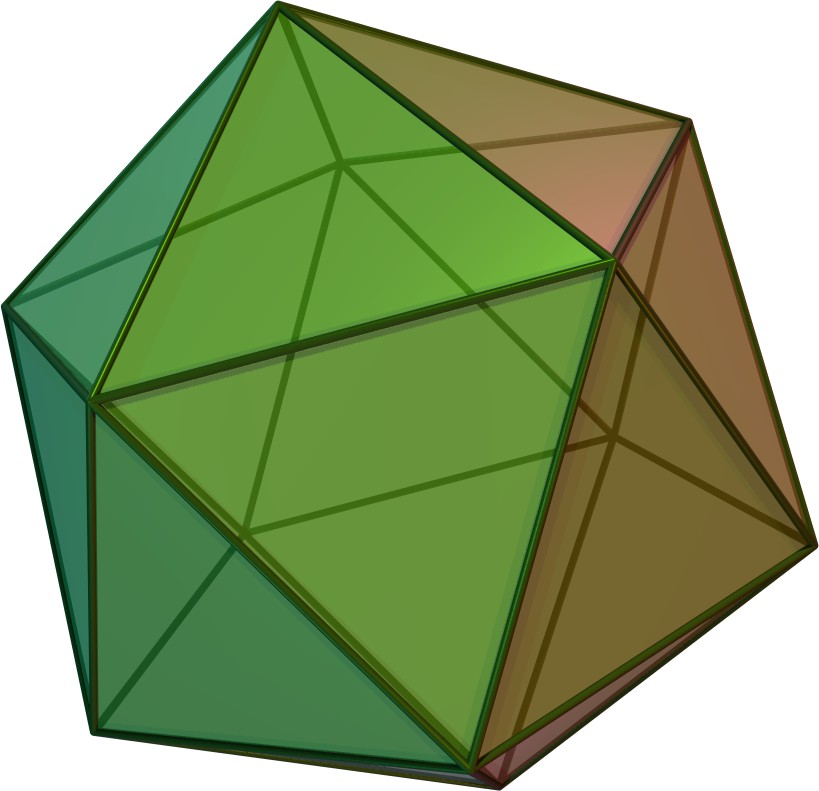
\includegraphics[width=.5\textwidth]{Icosahedron.jpg}
    \caption{正二十面体(\textit{Wikimedia Commons},按照CC BY-SA 3.0发布。\url{https://commons.wikimedia.org/w/index.php?title=File:Icosahedron.jpg&oldid=222275944})}
    \label{fig:icosahedron}
\end{figure}

为判断是否得到了正二十面体,我们可以将解得的res中各对电子之间的距离中最小的30个进行对比,如果它们都很接近$\frac{4}{\sqrt{10+2\sqrt{5}}} \approx 1.051\,462\,2242$,那么可以认为我们得到了一个正二十面体。

函数\texttt{distances<>()}会返回各对电子的间距组成的\texttt{vector}。
其基本基于\texttt{potential<>()}的代码,定义如下
{
    \linespread{1.0}
    \lstinputlisting[linerange=beg:distances-end:distances]{4_Thomson.cpp}
}
只是将\texttt{potential<>()}中的增加势能改为推入距离,并在最后排序。

随后,输出最小距离以及第30小的距离:
{
    \linespread{1.0}
    \lstinputlisting[linerange=end:12calc-end:icosahedron]{4_Thomson.cpp}
}
得到的结果分别是$1.051\,462\,071\,022\,363$与$1.051\,462\,360\,844\,809$。
两者都与$\frac{4}{\sqrt{10+2\sqrt{5}}} \approx 1.051\,462\,2242$十分接近,说明确实得到了一个正二十面体。

\subsection{求解小振动}
函数$f(\vb{x})$在极小值点$\vb{x}^*$附近(记$\vb{x} = \vb{x}^* + \vb{q}$)可展开为
\begin{equation}
    f(\vb{x}) = f(\vb{x}^*) + \frac{1}{2}\vb{q}^T\vb{H}(\vb{x}^*)\vb{q},
\end{equation}
其中黑塞矩阵
\begin{equation}
    \vb{H}(\vb{x}^*) = \qty{H_{ij}} = \qty{\pdv{f}{x_i}{x_j}}.
\end{equation}
显然,$\vb{H}(\vb{x}^*)$对称且在极小值处正定。
本问题中,由于三个额外自由度的存在,$\vb{H}(\vb{x}^*)$半正定,有三个特征值为0。

因此,在势能极小点附近,可展开为(使用爱因斯坦求和规则)
\begin{equation}
    V = \frac{1}{2}q_iV_{ij}q_j + V_0.
\end{equation}
加上动能展开式,能量守恒可写为
\begin{equation}
    \frac{1}{2}q_iV_{ij}q_j
    + \frac{1}{2}\dot{q}_iT_{ij}\dot{q}_j
    = C.
\end{equation}

两边对时间求导,考虑到$\qty{V_{ij}}$与$\qty{T_{ij}}$对称,可有
\begin{equation}
    \dot{q}_i
    \qty(V_{ij}q_j + T_{ij}\ddot{q}_j)
    = 0.
\end{equation}
又因为$\dot{q}$任意,可得
\begin{equation}
    V_{ij}q_j + T_{ij}\ddot{q}_j = 0.
\end{equation}
对于以$\omega$振动的本征简谐解,有
\begin{equation}
    V_{ij}q_j = \omega^2T_{ij}q_j,\quad
    \vb{V}\vb{q} = \omega^2 \vb{T}\vb{q},
\end{equation}
为一个广义本征值问题。

由于$\vb{V}, \vb{T}$都是半正定的,必均可对角化。我们假设$\vb{T}$可被正交矩阵$\vb{G}$对角化,有
\begin{equation}
    \vb{T} = \vb{G}^T\vb{T}\vb{G},
\end{equation}
那么
\begin{equation}
    \vb{G}\vb{V}\vb{G}^T\cdot\vb{G}\vb{q} = \omega^2\vb{D}_T\vb{G}\vb{T}.
\end{equation}

由于$\vb{T}$半正定,$\vb{D}_T$所有元素非负,可写为
\begin{equation}
    \vb{D}_T = \sqrt{\vb{D}_T}\sqrt{\vb{D}_T},
\end{equation}
有
\begin{equation}
    \sqrt{\vb{D}_T}^{-1}\vb{G}\vb{V}\vb{G}^T\sqrt{\vb{D}_T}^{-1}
    \cdot \sqrt{\vb{D}_T}\vb{G}\vb{q}
    = \omega^2\sqrt{\vb{D}_T}\vb{G}\vb{q}.
\end{equation}
问题变成了求
\begin{equation}
    \vb{V}' = \sqrt{\vb{D}_T}^{-1}\vb{G}\vb{V}\vb{G}^T\sqrt{\vb{D}_T}
\end{equation}
的所有特征值$\omega^2_i$。

本题中,
\begin{equation}
    T = \sum_{i}\frac{1}{2}(\dot{\theta}^2 + \dot{\phi}^2\sin^2{\theta}),
\end{equation}
$\vb{T}$已经是正定的,故只需求出黑塞矩阵$\vb{V}$,然后求$\vb{V}' = \sqrt{\vb{T}}^{-1}\vb{V}\sqrt{\vb{T}}$的本征值。

\subsubsection{黑塞矩阵}
前面在\autoref{ssec:grad} 已经求出了势能的梯度。
注意到,对梯度我们相当于得到了
\begin{equation}
    \pdv{q_i}\frac{1}{r} = \frac{A_i}{r^3}.
\end{equation}
那么黑塞矩阵便可拆成两部分
\begin{equation}\label{eq:hessian}
    \pdv{}{q_i}{q_j} \frac{1}{r}
    = \frac{3A_iA_j}{r^5} + \frac{1}{r^3}\pdv{A_i}{q_j}.
\end{equation}

黑塞矩阵的第一部分是现成的,下面着重说一下第二部分。
对于向量$\qty[\theta_i, \phi_i, \theta_j, \phi_j]$,黑塞矩阵的第二部分可写为(矩阵对称,仅列出上半部分)
\begin{equation}
    \frac{1}{r^3_{ij}}\mqty[
        \alpha& \beta&  \gamma& -\beta\\
        &   \delta& \epsilon&   -\delta\\
        &&  \alpha& -\epsilon\\
        &&& \delta
    ],
\end{equation}
其中
\begin{align}
    \alpha &{}= -\cos(\theta_i - \theta_j) + \sin{\theta_i}\sin{\theta_j}(1-\cos(\phi_i - \phi_j)),\\
    \beta &{}= -\cos{\theta_i}\sin{\theta_j}\sin(\phi_i - \phi_j),\\
    \gamma &{}= \cos(\theta_i - \theta_j) - \cos{\theta_i}\cos{\theta_j}(1-\cos(\phi_i - \phi_j)),\\
    \delta &{}= -\sin{\theta_i}\sin{\theta_j}\cos(\phi_i - \phi_j),\\
    \epsilon &{}= -\sin{\theta_i}\cos{\theta_j}\sin(\phi_i - \phi_j).
\end{align}

黑塞矩阵的计算函数如下
{
    \linespread{1.0}
    \lstinputlisting[linerange=beg:hessian_potential-end:hessian_potential]{4_Thomson.cpp}
}
其中大写字母开头的\texttt{Theta1}等变量即为 \eqref{eq:hessian} 中的$A_i$等。

由于之前计算极小值的时候固定了一个电子,在计算黑塞矩阵前要恢复这一自由度。
同时顺便将电子位型输出。
相应代码如下,完整的电子位型存储在\texttt{complete\_res}中。
{
    \linespread{1.0}
    \lstinputlisting[linerange=end:icosahedron-end:calc_hessian]{4_Thomson.cpp}
}

\subsubsection{本征值计算}
本人实现了双位移隐式QR算法,并用其计算本征值。
算法具体实现参见\texttt{misc/eigvals.h},下面仅简要说明一下思路。
首先介绍隐式QR定理\footnote{\url{http://math.ecnu.edu.cn/~jypan/Teaching/MatrixComp/slides_ch04_eig_nonsymm.pdf}}。

\begin{mythm}[隐式QR定理]
    设 $\vb{H} = \vb{Q}^T\vb{A}\vb{Q} \in \mathbb{R}^{n\times n} $是一个不可约上Hessenberg矩阵,其中$\vb{Q}\in \mathbb{R}^{n\times n}$是正交矩阵,则$\vb{Q}$的第 $2$ 至第$n$列均由$\vb{Q}$的第一列所唯一确定(可相差一个符号)
\end{mythm}

这样的话,就可以在实现QR算法的时候,只算出$\vb{Q}$的第一列,然后直接将原矩阵更改为下一个迭代,而不需要显式地进行QR分解,从而更为高效。

因此,本征值计算函数\texttt{eig\_vals()}的内部便是:
\begin{compactenum}
    \item 使用函数\texttt{hessenberg()}将矩阵变为海森堡矩阵;
    \item 使用隐式QR算法\texttt{\_eig\_hessenberg()}将海森堡矩阵变为块对角矩阵;
    \item 处理块对角矩阵的块对角元,给出所有实本征值以及复本征值对的实部与虚部。
\end{compactenum}
\texttt{eig\_vals()}返回一个存储本征值的\texttt{array}与标记复本征值位置的\texttt{vector}。
若本征值都是实的,则\texttt{vector}为空。

\subsubsection{计算结果}
由前面讨论,动能矩阵$\vb{T}$已经是对角的。
通过计算其平方根的逆,然后作用在$\vb{V}$的两侧,可以得到我们最终要求本征值的矩阵$\vb{V}'$。
{
    \linespread{1.0}
    \lstinputlisting[linerange=end:calc_hessian-end:calc_V_prime]{4_Thomson.cpp}
}
现在,\texttt{hessian}为$\vb{V}'$。

计算本征值,判断是否有复本征值。
如果没有,将本征值排序并输出。
{
    \linespread{1.0}
    \lstinputlisting[linerange=end:calc_V_prime-end:eigs]{4_Thomson.cpp}
}

运行结果表明,不存在复的本征值,所有本征值见\autoref{tab:omegas}。
表中也列出了小振动的角频率与简并度。
最小的角频率十分接近0,对应的是平动自由度,简并度为3。

\begin{table}
\centering
\caption{$N=12$时系统在极小值附近振动的角频率}
\label{tab:omegas}
\begin{tabular}{llc}
\toprule
\multicolumn{1}{c}{$\omega^2$} & \multicolumn{1}{c}{$\omega = \sqrt{\overline{\omega^2}}$} & 简并度 \\ \midrule
\multicolumn{1}{@{$-$}l}{6.266861164308746e$-$08} & \multirow{3}{*}{2.0735364285199273e$-$05} & \multirow{3}{*}{3} \\
1.332267629550188e$-$15 &  &  \\
6.395847630693958e$-$08 &  &  \\\midrule
0.9071635997689073 & \multirow{5}{*}{0.95245151613015140} & \multirow{5}{*}{5} \\
0.9071636643108395 &  &  \\
0.9071637783464412 &  &  \\
0.9071641902009776 &  &  \\
0.9071642202659546 &  &  \\\midrule
2.150595912152278 & \multirow{4}{*}{1.4664913062020637} & \multirow{4}{*}{4} \\
2.150596305870100 &  &  \\
2.150597197066894 &  &  \\
2.150597589575669 &  &  \\\midrule
5.160417841630242 & \multirow{3}{*}{2.2716553286841448} & \multirow{3}{*}{3} \\
5.160417964471208 &  &  \\
5.160417990915761 &  &  \\\midrule
6.605910534349911 & \multirow{4}{*}{2.5701967499033627} & \multirow{4}{*}{4} \\
6.605910921739608 &  &  \\
6.605911773209189 &  &  \\
6.605912103556530 &  &  \\\midrule
6.967665806026027 & \multirow{5}{*}{2.6396337464435122} & \multirow{5}{*}{5} \\
6.967665881324974 &  &  \\
6.967666491315732 &  &  \\
6.967666659903127 &  &  \\
6.967666738247202 &  &  \\ \bottomrule
\end{tabular}
\end{table}


% \appendix
% \renewcommand\chapterendname{}

% \chapter{\texttt{Misc}数值库接口}
% 本人将一些基本的矩阵类型以及相关算法写为\textsf{C++}头文件以方便调用。
本附录将简要介绍可用的接口。
所有的类以及函数均定义于命名空间\texttt{Misc}中,故下文不将\texttt{Misc::}显式写出。

可以通过引入\texttt{"Matrix\_Catalogue.h"}头文件引入所有矩阵类型以及有关运算符重载。
可以通过引入\texttt{"linear\_eq\_direct.h"}与\texttt{"linear\_eq\_iterative.h"}头文件调用矩阵的直接解法与迭代解法。

\section{矩阵}
所有的矩阵类型都继承自虚基类\texttt{template <typename T, size\_t R, size\_t C> class Base\_Matrix},其中模板参数\texttt{T}为数据类型,\texttt{R}, \texttt{C}分别为行数和列数。
注意,\textbf{所有矩阵规模参数都需要编译时指定}。
继承树为
{
\small
\begin{verbatim}
Base_Matrix<T, R, C> 虚基类
|Band_Matrix<T, N, M> 长宽为N,半带宽为M的带状矩阵
||Base_Half_Band_Matrix<T, N, M> 虚基类,长宽为N,半带宽为M
|||Low_Band_Matrix<T, N, M> 长宽为N,半带宽为M的下三角带状矩阵
|||Symm_Band_Matrix<T, N, M> 长宽为N,半带宽为M的对称带状矩阵
|||Up_Band_Matrix<T, N, M> 长宽为N,半带宽为M的上三角带状矩阵
|Base_Tri_Matrix<T, N> 虚基类,长宽为N
||Hermite_Matrix<T, N> 厄密矩阵,长宽为N
||Low_Tri_Matrix<T, N> 下三角矩阵,长宽为N
||Symm_Matrix<T, N> 对称矩阵,长宽为N
||Up_Tri_Matrix<T, N> 上三角矩阵,长宽为N
|Diag_Matrix<T, N> 对角矩阵,长宽为N
|Matrix<T, R, C> 一般矩阵,R行C列
|Sparse_Matrix<T, R, C> 稀疏矩阵;同时继承自std::array<std::map<size_t, T>, R>
\end{verbatim}
}

所有矩阵均提供的接口有
{
\linespread{1.0}
\begin{lstlisting}
Row<T, R, C> row(size_type pos);
const Row<T, R, C> row(size_type pos) const; // 返回某一行
Row<T, R, C> operator[](size_type pos);
const Row<T, R, C> operator[](size_type pos) const; // 同row()
Column<T, R, C> column(size_type pos);
const Column<T, R, C> column(size_type pos) const; // 返回某一列

const Transpose<T, C, R> trans() const; // 返回仅作为右值的转置

T &operator()(size_type row, size_type col);
const T &operator()(size_type row, size_type col); // 返回元素

using p_ta = T (*)[C];
p_ta data();
const p_ta data() const; // 返回内部存储数据的指针
constexpr size_type size() const; // 返回作为一个矩阵的元素个数
size_type data_size() const; // 返回存储的元素个数
size_type data_lines() const; // 返回存储的元素行数
constexpr size_type rows() const; // 返回矩阵行数
constexpr size_type cols() const; // 返回矩阵列数
std::pair<size_type, size_type> shape() const; // 返回矩阵形状
\end{lstlisting}
}

\texttt{row()}和\texttt{column()}方法返回\texttt{Row<T, R, C>}或\texttt{Column<T, R, C>}对象,可作为左值或右值。
可以通过\texttt{[]}下标运算符取或修改原矩阵的元素。

使用标准库类型\texttt{std::array<T, N>}作为矢量。

重载了矩阵间、矩阵与\texttt{Row}或\texttt{Column}或\texttt{array}之间的\texttt{*}运算符,可进行矩阵乘法。

所有矩阵均支持默认初始化,可以提供一个默认值。
如不提供,默认为0。

定义了一些类型间转换,可以把一些特殊的矩阵转化为更一般的矩阵。
比如,\texttt{Diag\_Matrix}可以转换为\texttt{Band\_Matrix}、\texttt{Up\_Tri\_Matrix}等等矩阵。

同时还定义了通过初始化器的列表初始化以便字面指定矩阵。
下面主要介绍一下这一初始化的使用。

\subsection{带状矩阵\texttt{Band\_Matrix}等}
需要沿对角线方向从右上到左下逐行输入,比如
{
\small
\begin{verbatim}
{
    {4, 6, 8, 3, 7},
    {3, 4, 7, 7, 4, 4},
    {2, 5, 5, 5, 2, 1, 7},
    {6, 3, 4, 4, 3, 6},
    {2, 7, 9, 2, 5}
}
\end{verbatim}
}
会得到矩阵\[
    \mqty(
        2&3&4&0&0&0&0\\
        6&5&4&6&0&0&0\\
        2&3&5&7&8&0&0\\
        0&7&4&5&7&3&0\\
        0&0&9&4&2&4&7\\
        0&0&0&2&3&1&4\\
        0&0&0&0&5&6&7
    ).
\]
输入格式错误会引发运行时错误。

对于半带状矩阵以及对称带状矩阵,初始化器的输入顺序为\textbf{从对角线向非零一侧}。

\subsection{三角矩阵\texttt{Base\_Tri\_Matrix}等}
水平从上到下依次输入半侧元素。
比如,
{
\small
\begin{verbatim}
{
    {4},
    {3, 4},
    {2, 1, 7},
    {6, 3, 4, 6},
    {2, 7, 9, 2, 5}
}
\end{verbatim}
}
会得到下三角矩阵\[
    \mqty(
        4&&&&\\
        3&4&&&\\
        2&1&7&&\\
        6&3&4&6&\\
        2&7&9&2&5
    )
\]
或对称矩阵\[
    \mqty(
        4&3&2&6&2\\
        3&4&1&3&7\\
        2&1&7&4&9\\
        6&3&4&6&2\\
        2&7&9&2&5
    ).
\]

但对应的上三角矩阵需要这样输入,
{\small
\begin{verbatim}
{
    {2, 7, 9, 2, 5},
    {6, 3, 4, 6},
    {2, 1, 7},
    {3, 4},
    {4}
}
\end{verbatim}
}
得到\[
    \mqty(
        2&7&9&2&5\\
        0&6&3&4&6\\
        0&0&2&1&7\\
        0&0&0&3&4\\
        0&0&0&0&4
    ).
\]

\subsection{对角矩阵\texttt{Diag\_Matrix}}
直接在一个初始化器列表内输入所有对角元即可。
也可通过提供一对迭代器初始化。

\section{矩阵的直接解法}
\texttt{"linear\_eq\_direct.h"}中主要是对矩阵进行分解的算法,提供\begin{enumerate}
    \item 三角矩阵回代 \texttt{back_sub()}
    \item LU分解 \texttt{lu\_factor()}
    \item LDL分解 \texttt{ldl\_factor()}
    \item Gauss-Jordan法求逆矩阵 \texttt{inv()};对特殊矩阵也会调用用其他算法
    \item 三对角矩阵追赶法 \texttt{tri\_factor()}
    \item Cholesky分解 \texttt{cholesky}
    \item 行列式计算 \texttt{det()}
\end{enumerate}

所有算法(除\texttt{det()})外均提供原处修改的接口与非原处修改接口。
如果仅传入待分解矩阵,那么会进行原处修改;如果也传入了输出矩阵,那么不会修改原矩阵。

\texttt{det()}函数会返回行列式的值。

\section{矩阵的迭代解法}
\texttt{"linear\_eq\_iterative.h"}中主要是对线性方程组进行迭代求解的算法,提供\begin{enumerate}
    \item Jacobi迭代法 \texttt{jacobi()}
    \item Gauss-Seidel迭代法 \texttt{gauss\_seidel()}
    \item 超松弛迭代法 \texttt{suc\_over\_rel()}
    \item 共轭梯度法 \texttt{grad\_des()}
\end{enumerate}

所有算法的接口是基本统一的,参数列表如下\begin{enumerate}
    \item \verb|const Base_Matrix<T, N, N> &in_mat| 系数矩阵
    \item \verb|const std::array<T, N> &in_b| 非齐次项
    \item \verb|std::array<T, N> &out_x| 解向量的初始值;输出的解向量
    \item \verb|T omega| 仅超松弛迭代使用的系数
    \item \verb|bool sparse = false| 是否为稀疏矩阵;如是,那么有优化
    \item \verb|size_t max_times = 1000| 最大迭代次数
    \item \verb|double rel_epsilon = 1e-15| 判停标准:残差与初始残差的1-范数之比小于此值时即停止
\end{enumerate}


\end{document}
